\section{Experiment}
\label{sec:experiment}

\subsection{Basic vs. Simulated Annealing}
\begin{frame}
	\frametitle{Cost}
	\begin{figure}[h]
		\centering
		\captionsetup[subfloat]{position=top}
		\hfill
		\subfloat[1 process, $T_{0}=1.0$]{
			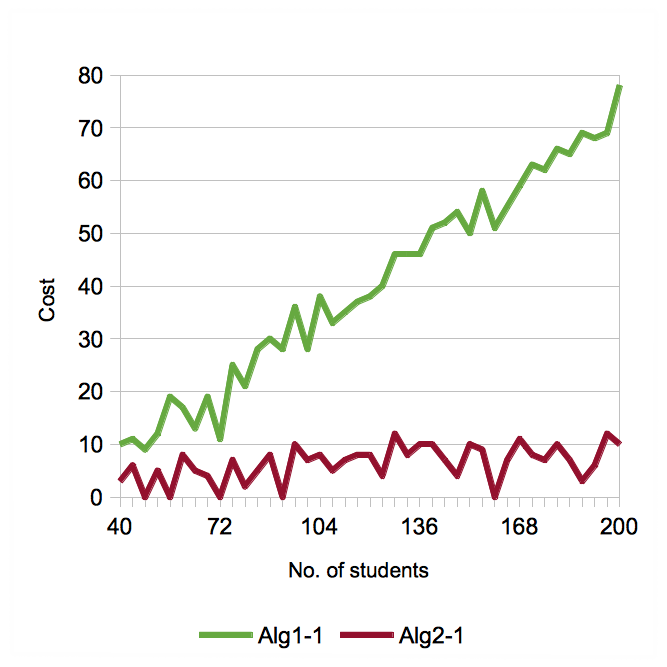
\includegraphics[width=0.45\textwidth]{slides/images/rand-01.png}
		}
		\hfill
		\subfloat[72 processes, $T_{0}=1.0$]{
			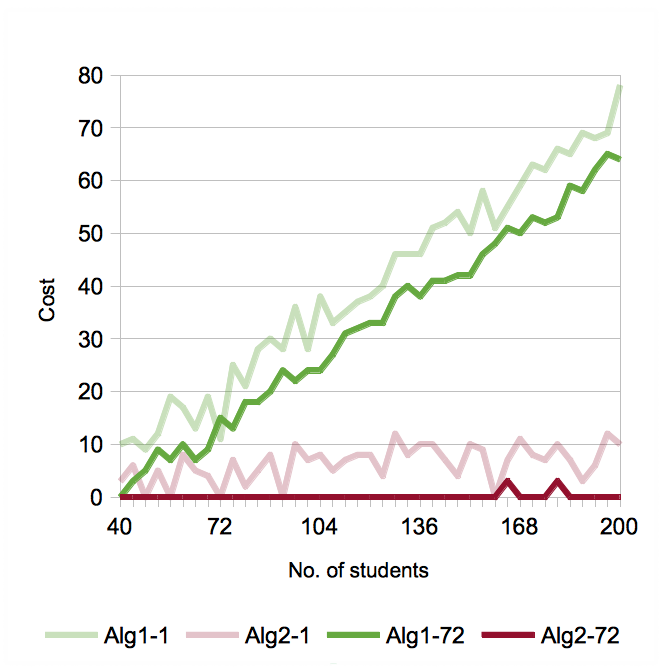
\includegraphics[width=0.45\textwidth]{slides/images/rand-72.png}
		}
		\hfill
		\ 
	\end{figure}
\end{frame}

\subsection{Initial temperature}
\begin{frame}
	\frametitle{Initial temperature}
	\begin{figure}[h]
		\centering
		\captionsetup[subfloat]{position=top}
		\hfill
		\subfloat[\smaller 1 process, $T_{0}=\{\;1.0\;,\;10.0\;,\;10^{4}\;\}$]{
			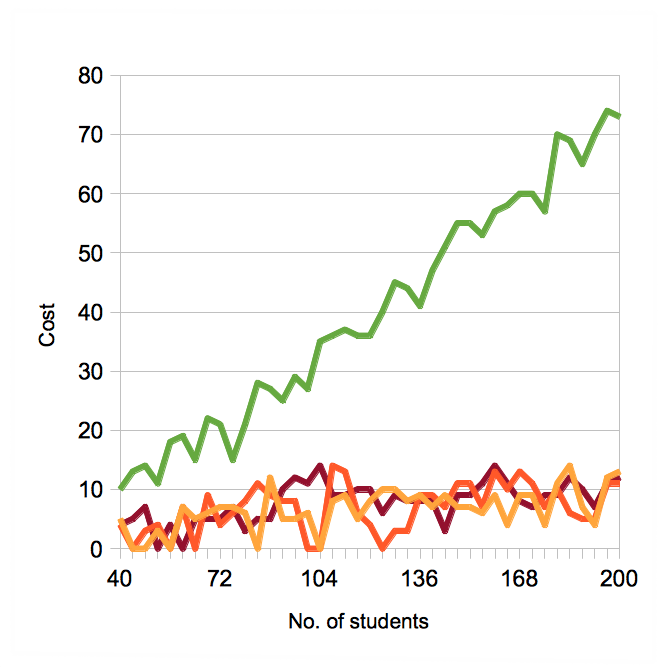
\includegraphics[width=0.45\textwidth]{slides/images/temp-cost.png}
		}
		\hfill
		\subfloat[\smaller 1 process, $T_{0}=\{\;1.0\;,\;10.0\;,\;10^{4}\;\}$]{
			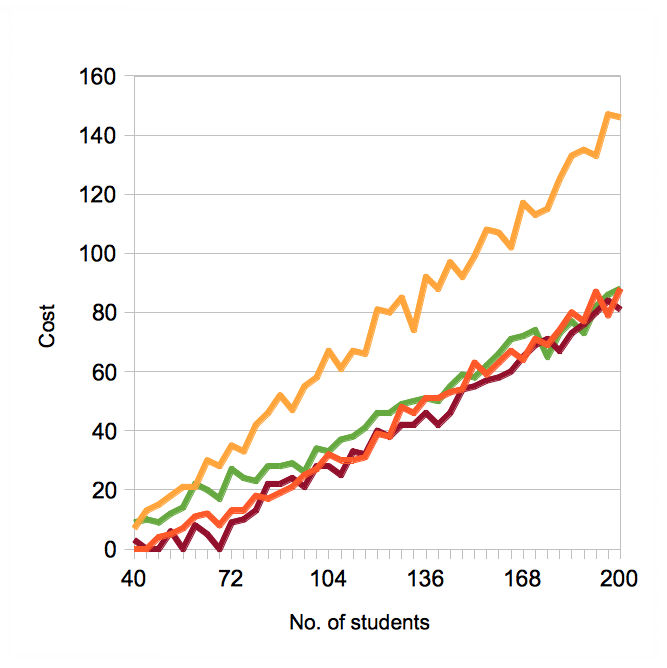
\includegraphics[width=0.45\textwidth]{slides/images/temp-cost-lim.png}
		}
		\hfill
		\ 

		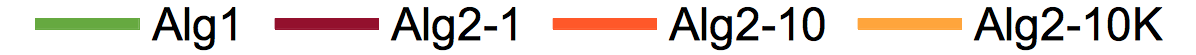
\includegraphics[width=0.6\textwidth]{slides/images/temp-leg.png}
	\end{figure}
\end{frame}